\section{Simulation of Controller}

For the simulation the controller was implemented in Simulink, and it operates alongside the autopilot described in chapter \ref{ch:simulation}. Since the controller will be used to control course using the rudder, the autopilot will be controlling all the other states and actuators.


\subsection{Controller Implementation}

The controller was implemented using a simple block diagram in Simulink, with desired course as input and rudder control as output. As a starting point for the controller tuning the control loop was simulated in an open loop. 

\subsection{Test Cases}


The altitude used when using a pushbroom sensor from an UAV for ground observation varies with what is being observed and the equipment used. When observing the vegetation, low-altitudes around $100$ m is often used (\cite{hymsySUOMALAINEN}, \cite{wheatLELONG}, \cite{lowRAMIREZ}). However, altitudes as high as $1900$ m has also been used to observe agricultural crops (\cite{mosaicASMAT}). In this paper simulations will be performed mainly at $100$ m. The FOV for the camera will be set to $19\degree$ (approximately the same as in \cite{hymsySUOMALAINEN}).

The controller has been tested in two different cases. The first case is a simple $45\degree$ turn in order to test the step response of the controller, and the response will be compared with a controller using ailerons to turn. In the second case the UAV will follow a ground path that is to be observed, and a comparison of the camera footprint made by the two controllers will be performed.


\subsection{Results: Step Response}

The step response of the controller is shown in figure \ref{fig:ratc_step_course}, together with the step response of a controller using the aileron to turn. The course angle $\chi$ reaches the desired $45\degree$ ($0.76$ $rad$) after about $80$ seconds. This is $20$ seconds after the aileron-controller starts to stabilize at $45\degree$, and while the aileron-controller is underdamped the rudder-controller is overdamped. Just after the step response has occured, the course angle for the rudder-controller starts off in the slightly wrong direction before it starts increasing.

\begin{figure}[]
    \centering
    \makebox[\textwidth][c]{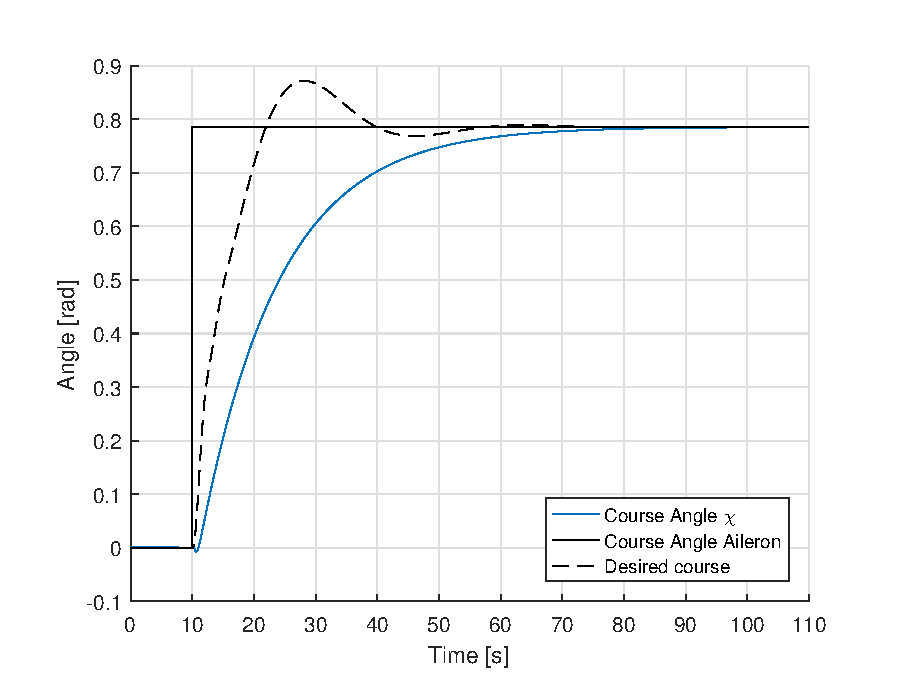
\includegraphics[width=1.0\textwidth, keepaspectratio=true]{../../results/controller/step/step_course.eps}}
    \caption{The step response of the course controller, compared to the course step response of a course controller using the ailerons.}
	\label{fig:ratc_step_course}
\end{figure}

\begin{figure}[]
    \centering
    \makebox[\textwidth][c]{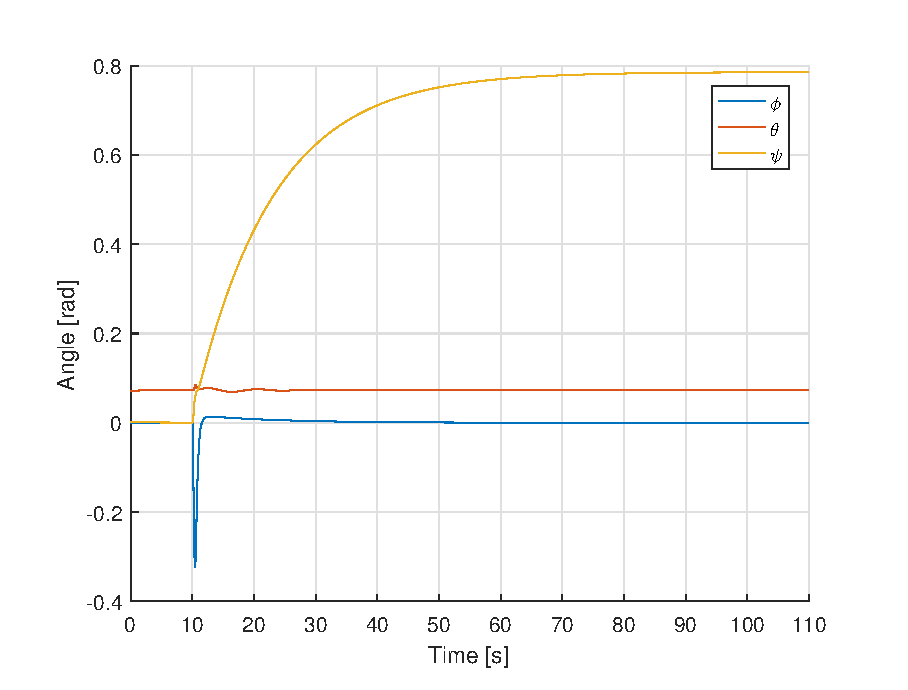
\includegraphics[width=1.0\textwidth, keepaspectratio=true]{../../results/controller/step/step_states.eps}}
    \caption{The attitude states of the UAV during the step response.}
	\label{fig:ratc_step_states}
\end{figure}

Figure \ref{fig:ratc_step_states} show that the pitch $\theta$ has only small variations when the step response occurs. When the step occurs the roll $\phi$ changes rapidly back and forth. This is because the deflection of the rudder actuator also induces a roll on the aircraft. This can also be seen on the inputs shown in figure \ref{fig:ratc_step_input}. At the time of the step both the aileron and the rudder increases rapidly, with an almost "mirrored" response.

\begin{figure}[]
    \centering
    \makebox[\textwidth][c]{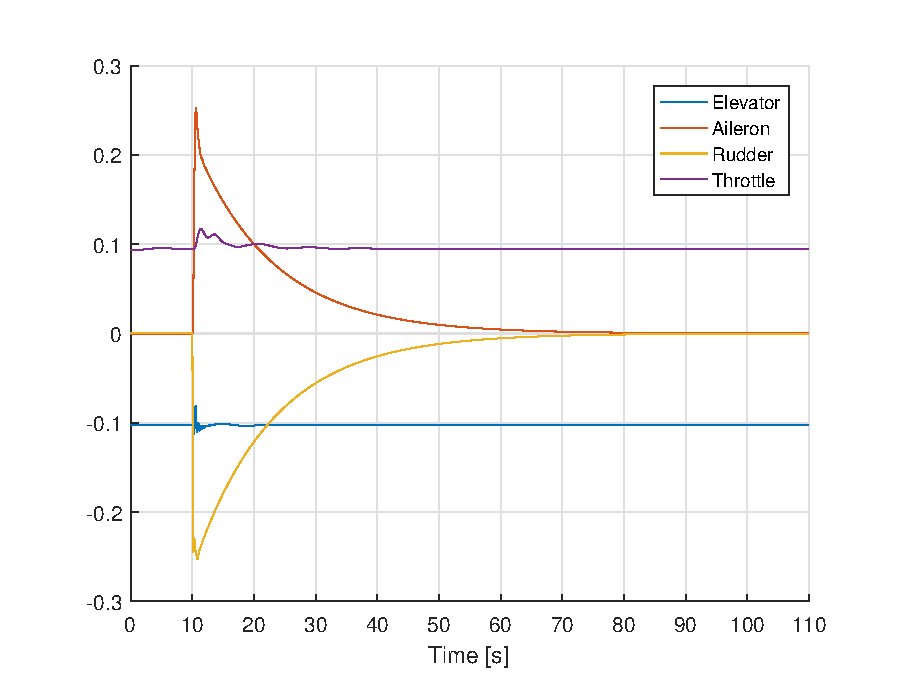
\includegraphics[width=1.0\textwidth, keepaspectratio=true]{../../results/controller/step/step_input.eps}}
    \caption{Input used during the step response. The input is given as a signal between $\pm1$.}
	\label{fig:ratc_step_input}
\end{figure}

The bode-plot in figure \ref{fig:ratc_bode} shows the frequency response of the rudder controller. The phase margin is $61.2\degree$ and since the pase never goes below $-180\degree$, this is a stable system (ch. 8.4.7, \cite{regBALCHEN}). This tuning was achieved with $\zeta$ set to $0.6$ and $\omega_n$ set to $3.5$, which corresponds to a $k_p$ of $-0.3574$ and a $k_d$ of $0.2090$.

\begin{figure}[]
    \centering
    \makebox[\textwidth][c]{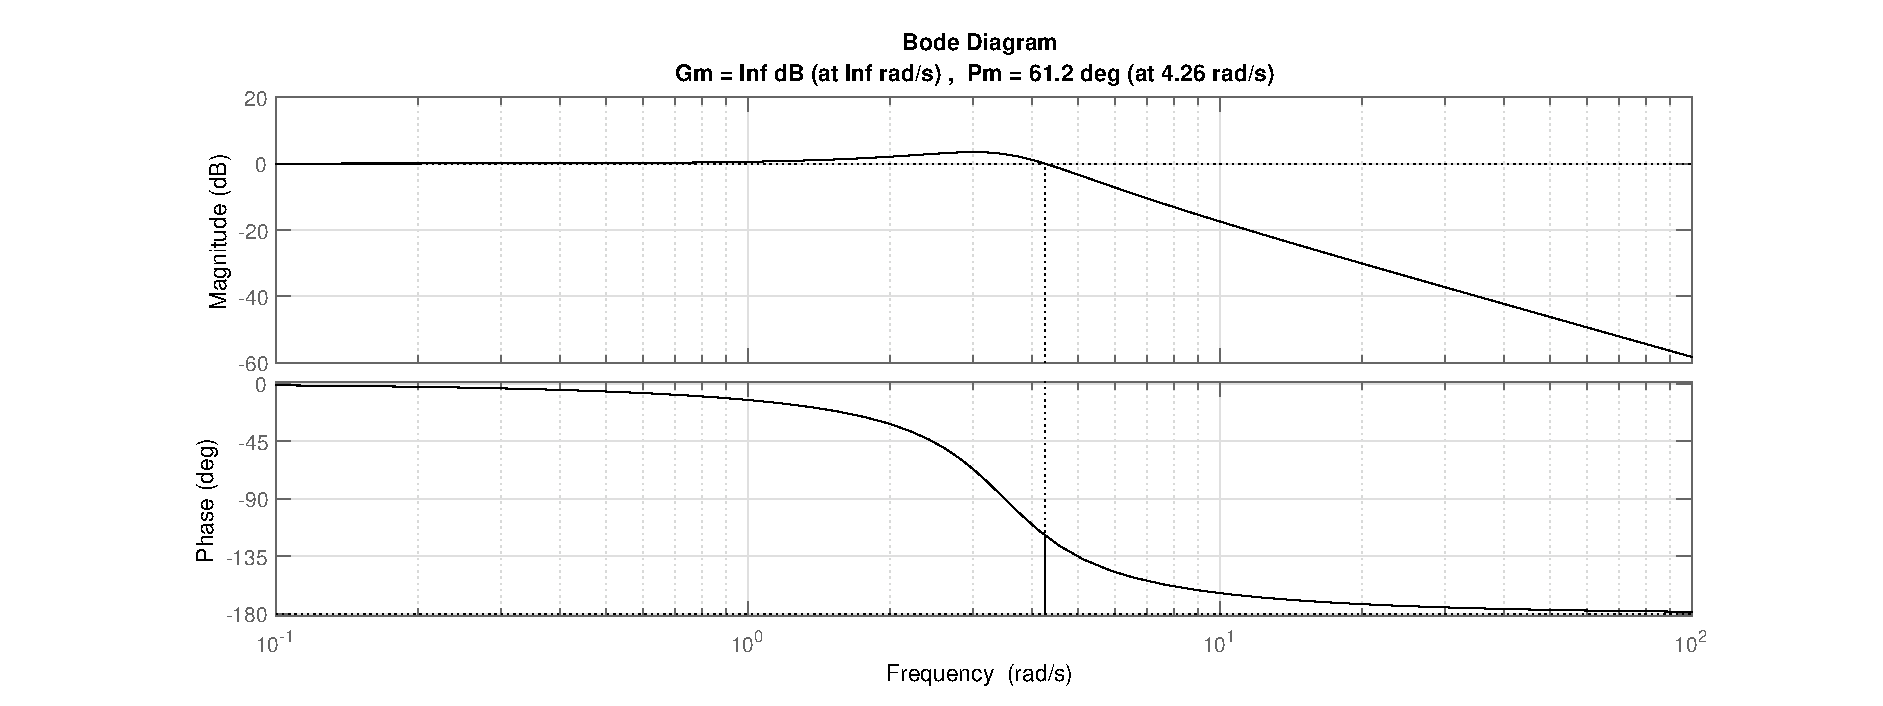
\includegraphics[width=1.6\textwidth, keepaspectratio=true]{../../results/controller/step/bode.eps}}
    \caption{The camera footprint during simulation of the first path.}
	\label{fig:ratc_bode}
\end{figure}


\subsection{Results: Path}

The path flown and the corresponding camera footprint when the course is controlled using the rudder is shown in figures \ref{fig:ratc_path_hundred} and \ref{fig:ratc_comp_hundred}. The figures show that the ground path remains within the camera footprint when the ground path is straight, but the camera footprint shifts away from the ground path during turns, except from the first, gentle turn. The roll that is induced by the rudder that was seen in the step response, is visible on the camera footprint as well. At the beginning of each turn there are a small "NUDGE" in the footprint, but none of them moves the camera outside the observation path.

\begin{figure}[]
    \centering
    \makebox[\textwidth][c]{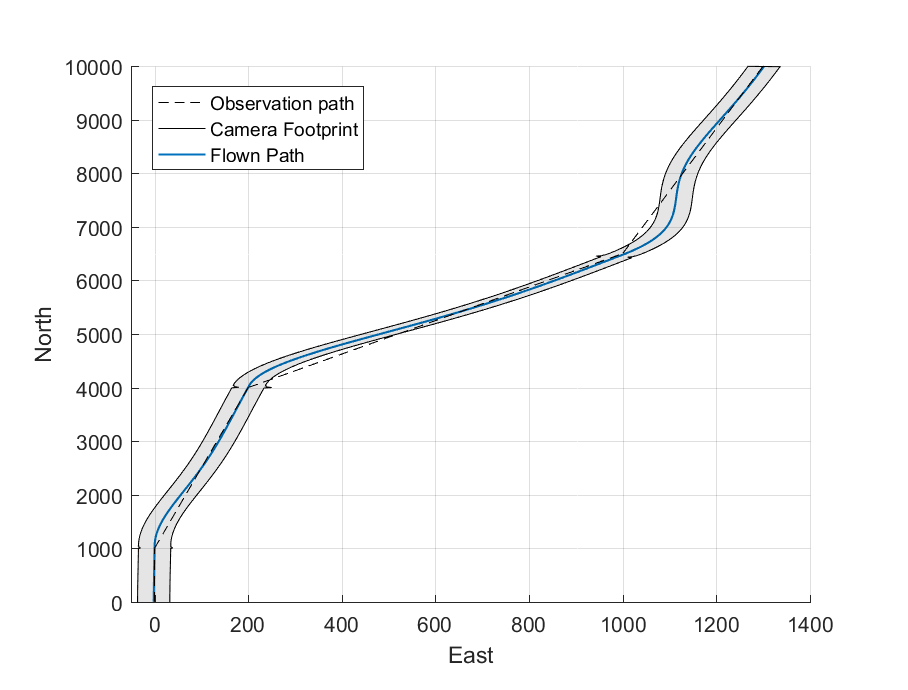
\includegraphics[width=1.0\textwidth, keepaspectratio=true]{../../results/controller/path/ratc_path_hundred.eps}}
    \caption{The path flown and the camera footprint when following the path using the rudder controller. Altitude is $100$ m.}
	\label{fig:ratc_path_hundred}
\end{figure}

\begin{figure}[]
    \centering
    \makebox[\textwidth][c]{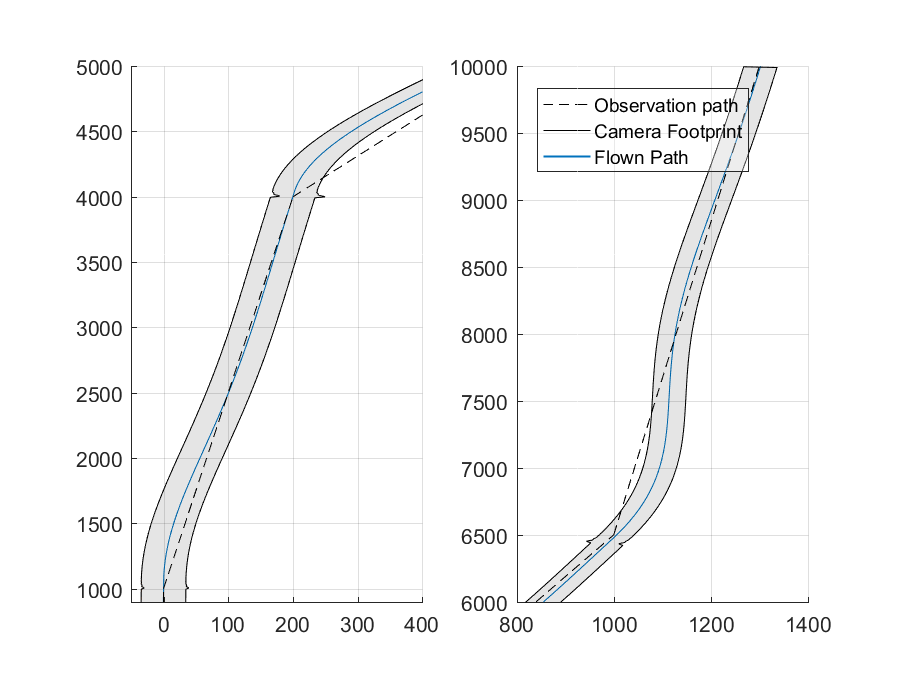
\includegraphics[width=1.0\textwidth, keepaspectratio=true]{../../results/controller/path/ratc_comp_hundred.eps}}
    \caption{Detailed view of the path flown and the camera footprint when following the path using the rudder controller. Altitude is $100$ m.}
	\label{fig:ratc_comp_hundred}
\end{figure}

Figures \ref{fig:aotc_path_hundred} and \ref{fig:aotc_comp_hundred} shows the flight of the UAV when using the aileron to change the course. The obsevation path is within the camera footprint almost throughout the flight, but the edge of the camera footprint is close to the observation path at multiple times. At the beginning of every turn there is rapid shift in the camera footprint because of an abrupt roll change, and after every turn the roll of the aircraft oscillates back and forth before it settles.

\begin{figure}[]
    \centering
    \makebox[\textwidth][c]{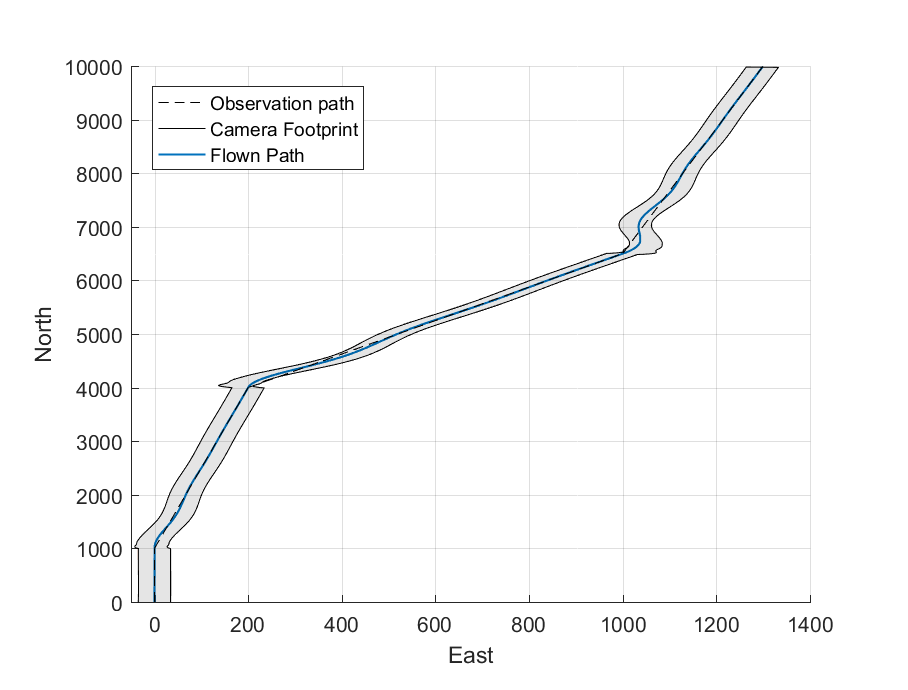
\includegraphics[width=1.0\textwidth, keepaspectratio=true]{../../results/controller/path/aotc_path_hundred.eps}}
    \caption{The path flown and the camera footprint when following the path using the aileron controller. Altitude is $100$ m.}
	\label{fig:aotc_path_hundred}
\end{figure}

\begin{figure}[]
    \centering
    \makebox[\textwidth][c]{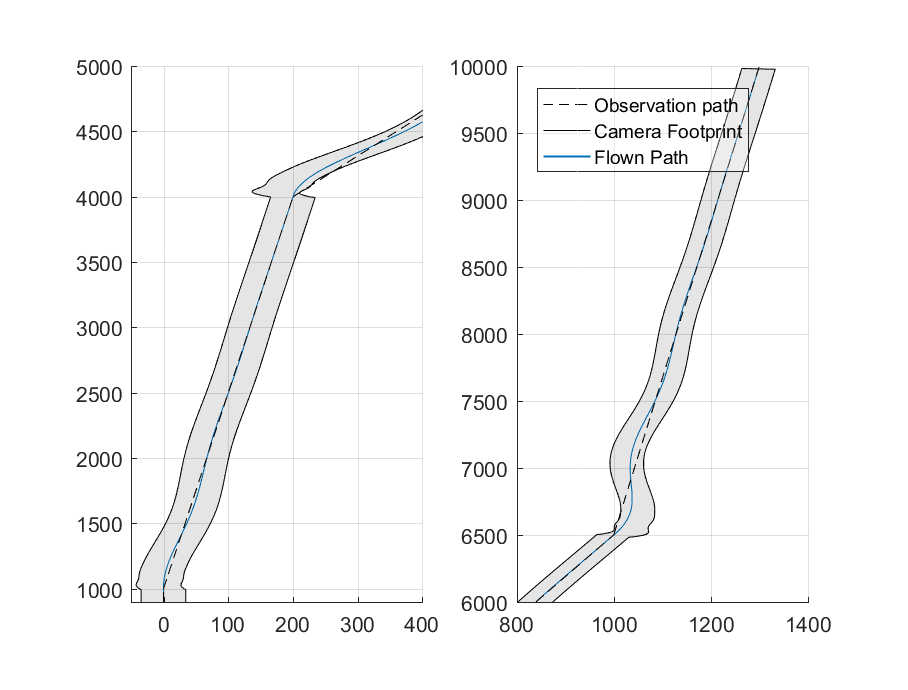
\includegraphics[width=1.0\textwidth, keepaspectratio=true]{../../results/controller/path/aotc_comp_hundred.eps}}
    \caption{Detailed view of the path flown and the camera footprint when following the path using the aileron controller. Altitude is $100$ m.}
	\label{fig:aotc_comp_hundred}
\end{figure}

The camera footprint made by both of the controllers is shown together in figure \ref{fig:ratc_aotc_comparison}. The figure shows that the camera footprint of the aileron controller oscillates more than the footprint of the rudder controller, but it doesn't necessarily move further away from the observaton path. At the beginning of the turns both of the controllers causes a "NUDGE" in the camera footprint in opposite directions. The "NUDGE" of the aileron controller is bigger and remains longer than the "NUDGE" for the rudder controller.

\begin{figure}[]
    \centering
    \makebox[\textwidth][c]{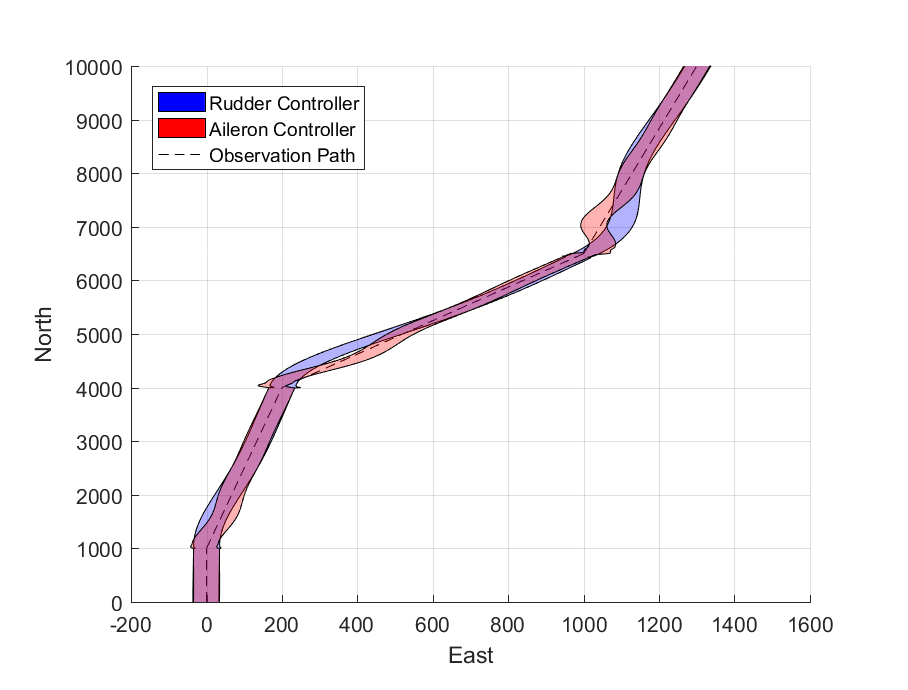
\includegraphics[width=1.0\textwidth, keepaspectratio=true]{../../results/controller/path/comparison.eps}}
    \caption{A comparison of the camera footprints of the two controllers. Altitude is $100$ m.}
	\label{fig:ratc_aotc_comparison}
\end{figure}


\subsection{Discussion}

The step response of the aileron controller was the best and the simulations of the path show that quick response is a favorable trait when tracking a path. However, the simulations show that a quick response is not the most important trait when performing ground observation. The quick response comes at the expense of lateral deviation in the camera footprint caused by the roll. The slower response of the rudder controller reduces the sideway changes in the camera footprint, but the slower response also causes the observation path to move out of the observation path because the controller doesn't manage to keep up with the path.

Both of the controllers causes abrupt changes in the roll of the aircraft, which again causes a lateral shift in the camera footprint. This is where the rudder controller performs better than the aileron controller. While the aileron controller is underdamped and the roll oscillates, the rudder controller makes a smoother course changes with the little nudge at the beginning of the turn as the only significant change in roll or pitch.

Even though the camera footprint made by the aileron controller covers the observation path for a larger portion of the path than the footprint made by the rudder controller, it does not necessarily result in better images. The camera footprint of the aileron controller has more lateral movement than the rudder controller has, and the images shot in sections with a lot of lateral movement is most likely not as clear as they should be. The rudder controller do have some small, lateral jerks in the camera footprint as well, but it is possible that these can be made even smaller with better tuning of both the rudder controller and the aileron controller that keeps the wings level. The simulations show that the rudder controller performs much better in this area.

It is worth noting that the path simulated in this section was designed to test the rudder controller, and the two last turns was chosen so that the rudder controller would not be able to follow them with high enough precision so that the observation path stays within the camera footprint. The first turn can therefore be seen as a "maximum turn angle" that the rudder controller produced in this paper can track. In addition the path planner used for both of the controllers was not designed for ground observation. This means that the path follower does not tell the controllers to change course for the next waypoint until the UAV has passed the current waypoint. In a situation where ground observation is the goal, the path follower should start changing course for the next waypoint before the current waypoint has been passed.

\begin{figure}[]
    \centering
    \makebox[\textwidth][c]{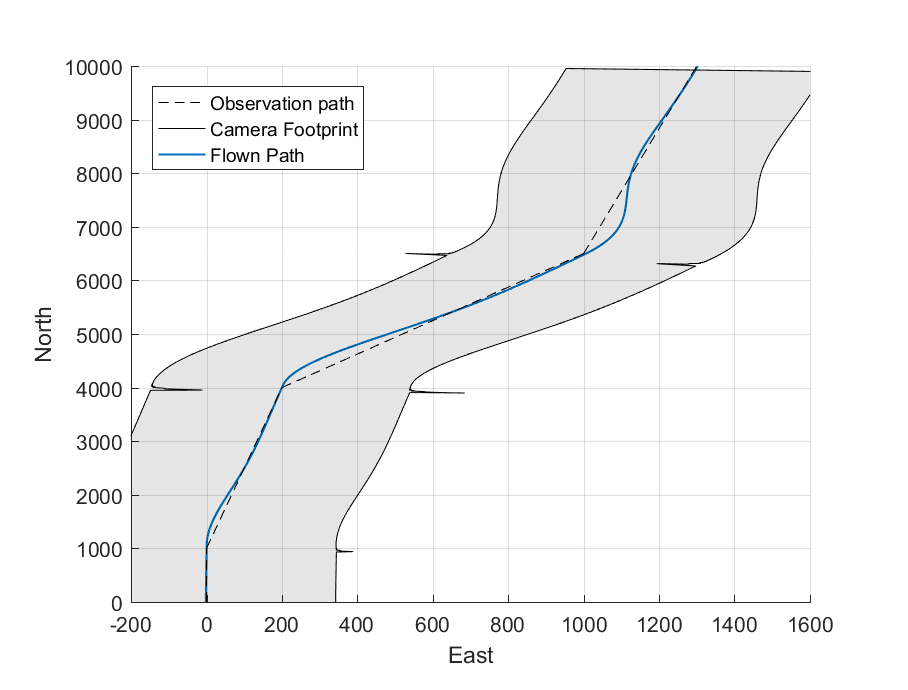
\includegraphics[width=1.0\textwidth, keepaspectratio=true]{../../results/controller/path/ratc_thousand.eps}}
    \caption{The camera footprint of the rudder controller flown at an altitude of $1000$ m.}
	\label{fig:ratc_thousand}
\end{figure}

The controllers were also simulated when flying at an altitude of $1000$ m, and the resulting path for the rudder controller is shown in figure \ref{fig:ratc_thousand}. The camera footprint is much larger, and therefore covers the observation path at all times. However, the lateral changes are still visible from this altitude and they are also amplified, meaning that increased altitude does not lead to more usable images. The results for the aileron controller were matching.